\documentclass[10pt, titlepage, oneside, a4paper]{article}
%\documentclass{book}


\usepackage[T1]{fontenc}
\usepackage[english]{babel}
\usepackage{amssymb, graphicx}
\usepackage{fancyhdr}
\usepackage{listings}
\usepackage{epstopdf}


\addtolength{\textheight}{20mm}
\addtolength{\voffset}{-5mm}

\renewcommand{\sectionmark}[1]{\markleft{#1}}
%\renewcommand{\chaptermark}[1]{%

%\markboth{#1}{}} \renewcommand{\sectionmark}[1]{%
%\markright{\thesection\ #1}}

% \Section ger mindre spillutrymme, anv?nd dem om du vill
\newcommand{\Section}[1]{\section{#1}\vspace{-8pt}}
\newcommand{\Subsection}[1]{\vspace{-4pt}\subsection{#1}\vspace{-8pt}}
\newcommand{\Subsubsection}[1]{\vspace{-4pt}\subsubsection{#1}\vspace{-8pt}}
	
% appendices, \appitem och \appsubitem ?r f?r bilagor
\newcounter{appendixpage}

\newenvironment{appendices}{
	\setcounter{appendixpage}{\arabic{page}}
	\stepcounter{appendixpage}
}{
}

\newcommand{\appitem}[2]{
	\stepcounter{section}
	\addtocontents{toc}{\protect\contentsline{section}{\numberline{\Alph{section}}#1}{\arabic{appendixpage}}}
	\addtocounter{appendixpage}{#2}
}

\newcommand{\appsubitem}[2]{
	\stepcounter{subsection}
	\addtocontents{toc}{\protect\contentsline{subsection}{\numberline{\Alph{section}.\arabic{subsection}}#1}{\arabic{appendixpage}}}
	\addtocounter{appendixpage}{#2}
}

\def\inst{Teknik och Naturvetenskap}
\def\course{Fluid Simulation}
\def\pretitle{TNM085 Modelleringsprojekt}
\def\title{TNM085 MODELLERINGSPROJEKT}
\def\graders{Anna Lombardi}


% om du vill referera till katalogen d?r dina filer ligger kan du 
% anv?nda \fullpath som kommer att vara "~username/edu..." o.s.v.
\begin{document}

	% skapar framsidan (om den inte duger: g?r helt enkelt en egen)
	
	\begin{titlepage}

		\thispagestyle{empty}
		
		\begin{large}
			\begin{tabular}{@{}p{\textwidth}@{}}
			
				\textbf{LINK�PINGS UNIVERSITET\hfill} \\
				\textbf{Institutionen f�r \inst} \\
			\end{tabular}
		\end{large}
		\vspace{50mm}
		\begin{center}
			\LARGE{\pretitle} \\
			\huge{\textbf{\course}}\\
			\vspace{10mm}
			
			\vspace{15mm}
			\normalsize\today
			\vspace{15mm}
			
			\begin{large}
			Robert Novo, robno767@student.liu.se\\
			Martin Person, marpe357@student.liu.se\\
			Mattias Persson, matpe621@student.liu.se\\
			Johannes Ullstr�m, johul223@student.liu.se\\
			\end{large}
			
			\vfill
			\large{\textbf{Examiner}}\\
			\mbox{\large{\graders}}
		\end{center}
	\end{titlepage}

	\begin{abstract}
	\end{abstract}

	% fixar sidfot och sidhuvud
	\lfoot{\footnotesize{\name\course}}
	\lhead{\nouppercase\sc\footnotesize\title}
	\rhead{\nouppercase{\sc\footnotesize}}
	\pagestyle{fancy}
	\renewcommand{\headrulewidth}{0.2pt}
	\renewcommand{\footrulewidth}{0.2pt}

	% skapar inneh�llsf?rteckning.
	% T?nk p� att k?ra latex 2ggr f?r att uppdatera allt
	\tableofcontents
	
	\newpage
	
	\addtocontents{toc}{\protect\thispagestyle{empty}}
	\listoffigures    % chapter with the list of figures
	\addtocontents{lof}{\protect\thispagestyle{empty}}
	\listoftables     % chapter with the list of tables
	\addtocontents{lot}{\protect\thispagestyle{empty}}
	% och l?gger in en sidbrytning
	\newpage

	\pagenumbering{arabic}

	% i Sverige har vi normalt inget indrag vid nytt stycke
	\setlength{\parindent}{0pt}
	% men d?remot lite mellanrum
	\setlength{\parskip}{10pt}

\section{Introduction}
Simulation of different physical phenomena is increasingly used within several fields including such diverse areas as various scientific researches and the entertainment industry, for instance in gaming development or special effects in movies. Consequently, we find that the simulation of fluids would be an exciting and important region to explore. The aim of this project is to program an interactive application which simulates fluids in 3D.

\subsection{Usage}
	\subsubsection{Computer games}
	In computer games of today the player is likely to encounter some sort of fluid being simulated, whether it be water, smoke etcetera. In order to improve rendering speed and visual quality of the simulation, some physical details are sacrificed. To interact with fluids in game the simulation is usually done by graphic card calculations.
	
	\subsubsection{Movies}
	On the contrary to computer games, where the focus lies in rendering speed, the most important factor of fluid simulations in movies is its visual appearance. Real-time rendering is not necessary in movies, thus enabling heavier calculations, should that be required for the visual appearance.
	
\section{Methods}
Below we present the methods used in the project.

	\subsection{Navier-Stokes equations}
	A well-used method for description of fluids is the Navier-Stokes equations which were formulated by Claude-Louis Navier and George Gabriel Stokes. Navier-Stokes utilized Newtons second law to describe flows of fluids that is steady and generated a series of differential equations [1]. The Navier-Stokes equations made it possible to illustrate how magnitudes like pressure, density, viscosity relates and affect the fluid.

	\subsection{SPH, Smoothed Particle Hydrodynamics}
	Smoothed Particle Hydrodynamics (SPH), as developed by Lucy and Gingold, is originally a method of simulating astrophysical problems, but is sufficient enough to simulate any kind of fluid. In an article by M�ller, Charypar and Gross (2003), the authors present a further development of the method. M�ller et al concludes that in order to determine the movement of every particle you will need to include the following forces: mass, pressure, viscosity, surface tension and gravity. You will also need to incorporate a smoothing kernels method, which regulates the SPH's stability, accuracy and speed. According to SPH, a scalar quantity A is interpolated at location r by a weighted sum of contributions from all particles:
	
	
\begin{equation}
	A_{S}(\textbf{r}) = {\sum_{j}} m_{j} \frac{A_{j}}{\rho_{j}} W(\textbf{r}-\textbf{r}_{j},h)
\label{eq:}
\end{equation}

Where $m_{j}$ is the mass and $\rho_{j}$ is the density of particle $j$. The function $W$ is a weight function called a smooth kernel.
	
	\subsection{Particles}

	\subsection{Marching cubes}
Marching cubes is an algorithm for making particles "melt" together and construct a surface or so called "mesh". Developed by Cline and Lorensen in 1987, at the time working for General Electric Company, marching cubes uses 256 cube configurations to represent every way the mesh could cross the cube. Utilizing symmetries can reduce the configurations to 15 unique patterns.

		\begin{figure}[htb]
		\begin{center}
			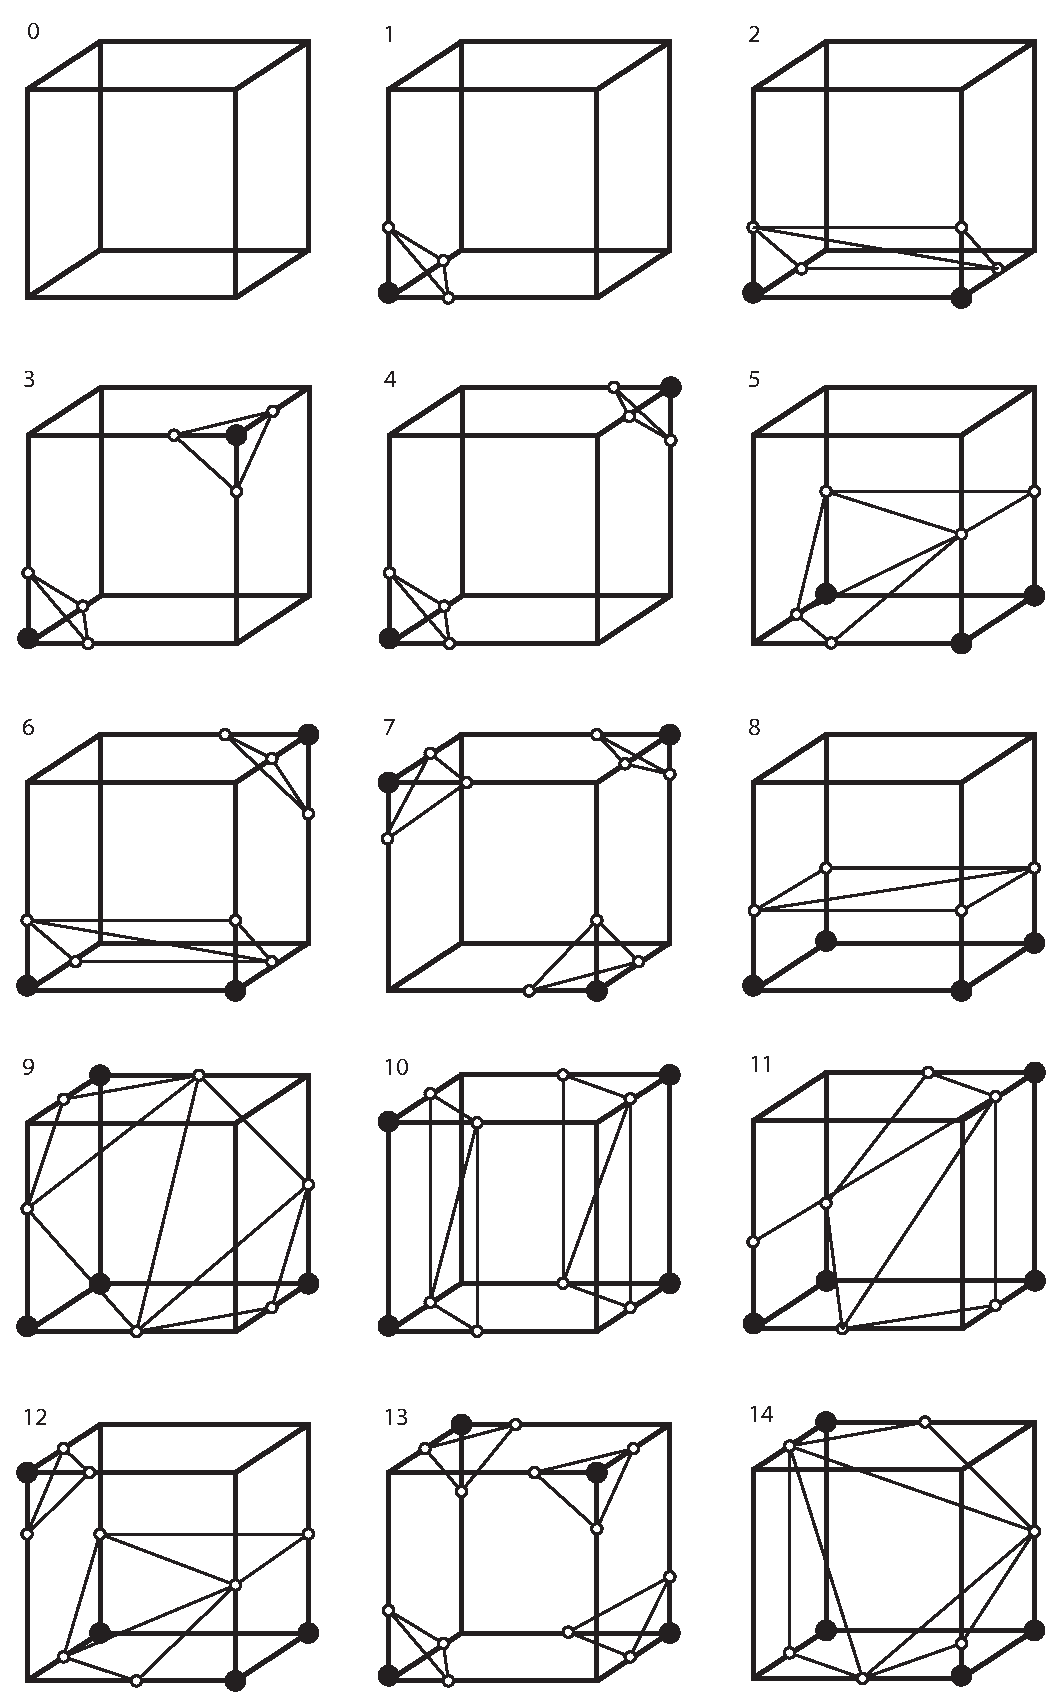
\includegraphics[scale=0.5]{Figures/marching_cubes.eps}
				\caption{Marching cubes}
		\end{center}
			\label{MarchingCubes}
		\end{figure}
		
	\subsection{C\#/.Net and XNA}
	The executable files for this project was written the programming language C\# and Microsoft .NET was utilized as a framework. To make graphics easier to display the environment Microsoft XNA was used. 

\section{System description}

	\subsection{System}
	The system that we have built is a fluid represented by particles. Different forces act on the particles which causes them to move the way they do. Fluids are materials that are being deformed under forces. They are commonly known to be liquids but fluids are also gases. Our model is capable simulating a gas like substance. However, the focus was mainly on creating a liquid. Normally, a simulation system is described with a bond graph or block diagram. In our case though, because this is a particle based fluid simulation, which requires quite a lot of particles to look like liquid, it is hard.

	
	%\subsection{Model}

	\subsection{Physical history}
	One method to describe how fluids behave (describe the motion of substances) is the Navier-Stokes equations, named after Claude-Louis Navier and George Gabriel Stokes. This method is used for this project.

	As seen in the equation below, the physical quantities used are pressure, density and viscosity.
	
	
	\begin{equation}
	\rho\left(\frac{\partial v}{\partial t} + v \cdot\nabla v\right) = -\nabla p + \rho g	 + \mu\nabla^{2}v
\label{eq:}
\end{equation}

This equation is then simplified, as suggested by M�ller03 to:

\begin{equation}
\textbf{a}_{i} = \frac{d\textbf{v}_{i}}{dt} = \frac{-\nabla p_{i} + \rho_{i}\textbf{g}+\mu \nabla^{2}\textbf{v}_{i}}{\rho_{i}}
\label{eq:}
\end{equation}

Where $-\nabla p_{i}$ is force due to pressure, $\rho_{i}\textbf{g}$ is external forces such as gravity and $\mu\nabla^{2}\textbf{v}_{i}$ is force due to visosity.

	\subsection{Pressure}
		
	\subsection{Density}
The first step in the simulation is computing the particle densities. By substituting $A$ in equation x with the particle density $\rho$, we get:
\begin{equation}
	\rho_{S}(\textbf{r}) = {\sum_{j}} m_{j}W(\textbf{r}-\textbf{r}_{j},h)
\label{eq:}
\end{equation}
The smoothing kernel used for calculating the density in this simulation was the $W_{poly6}$ kernel, designed by M�ller03.

\begin{equation}
	\rho_{S}(\textbf{r}) = {\sum_{j}} m_{j}W(\textbf{r}-\textbf{r}_{j},h)
\label{eq:}
\end{equation}
	
	\subsection{Viscosity}
	Viscosity is caused by friction which converts the particle's kinetic energy to heat.
	The viscosity is calculated by looking at the force in the gradient of the neighbors of each particle.
	
	\subsection{Force simulation}
	The sum of all forces that act on the particles is used for the final calculation that will actually move a particle. The force is recalculated according to Newtons 2nd law to acceleration. The current acceleration is multiplied with a predefined timestep and added to the current velocity. The new velocity is multipled with the same predefined timestep, which gives the movement ant therefore the new position of the particle.
	\subsection{Collision Handling}
	The collision handling performed in this simulation is fairly simple. A bound is defined in which the fluid can exist. After a particle's new position is calculated, the program checks if it is within the acceptable bounds or not. If the particle's position is not within the defined area, the velocity and acceleration of the particle is inverted, otherwise nothing changes.
	
		
\section{Implementation}
	

	\subsection{Rendering}
	The simulation is rendered using the benefits of XNA... bla bla.
\section{Results}

\section{Conclusion}
- Producing realistic simulation of fluids is very difficult. It is also hard to define what a "good" simulation is. There are several other simulations, often published as short demonstration films that are pre-rendered and not interactive. An example of that is the result of Beaudoin, Clavet and Poulin (2005). Beaudoin et al produces stunning visuals and the clip has gotten 23 956 views on youtube.com (2011-03-09) which certainly could be rubricated as "good". With that in mind we think that our own result is good. We have succeeded in reaching the aim of our project.

What could have been done differently?
-  One could consider if the same, or better, result could be accomplished if another environment had been chosen as a platform for the project. For example if we have had chosen OpenGL instead of XNA. It was also possible to have used other methods to reach our goal. One of the most important reasons why we chose to use SPH was that there were quite a lot of resources available on the subject. At one point we were considering using point splatting (M�ller at alt, 2003) instead of marching cubes. But we quickly realized that point splatting generally uses 10.000 to 100.000 particles, which would have demanded significantly more CPU-power, since we only used up to 2000 particles in our system.
If we wanted to continue developing the software, what would we have done?
- In an ongoing development of the project we would concentrate our efforts to implement the NVIDIA engine CUDA, Compute Unified Device Architecture, to the project. CUDA uses the inbuilt graphics card of the computer to calculate simple computations and unburden the CPU. Doing this will improve the "speed" of the simulation, i.e. the number of frames/second. We would also do more collision handling. We could for example have a static object in the glass cube that the fluid would have to interact with.

\end{document}